\chapter{Normalising the Typed Lambda Calculus}
\label{chap:typednbe}

In this chapter, we translate an Agda implementation of NbE developed by Andras Kovacs \cite{AgdaNbe} for the STLC into Haskell.

\section{Target Syntax}

% TODO: Colour for polymorphic type variable in certain blocks

We construct the set of the simply typed normal terms \code{NormalForm} by combining the approach seen for the untyped terms in Chapter \ref{chap:untypednbe} with the GADT syntax from Chapter \ref{chap:typedlamadacalculus} to ensure \code{NormalForm}'s inhabitants are well-typed.

\begin{lstlisting}
    data NormalForm :: [Ty] -> Ty -> * where
        NormalNeutral :: NeutralForm ctx ty -> NormalForm ctx ty
        NormalLam     :: NormalForm (arg : ctx) result -> NormalForm ctx (arg :-> result)    

    data NeutralForm :: [Ty] -> Ty -> * where
        NeutralVar :: Elem ctx ty -> NeutralForm ctx ty
        NeutralApp :: NeutralForm ctx (arg :-> result) -> NormalForm ctx arg 
                   -> NeutralForm ctx result

\end{lstlisting}

% TODO: Justify why V has context (need to reify, example, normalise identity), describe what we need



% TODO: First evaluation problem - returning correct semantic context, lambda has different syntax
% - Solved for us by Andras

% TODO: Correspondence with untyped env, Motivate need for tracking type, ctxV

\section{Order Preserving Embeddings}

In the lambda case of \code{eval}, NbE evaluates the body of the lambda in a stronger context where a new bound variable is introduced (as seen in Chapter \ref{chap:untypednbe}). To continue the evaluation of the body ...

\begin{lstlisting}
    data OPE :: [Ty] -> [Ty] -> * where
        Empty :: OPE '[] '[]
        Drop  :: OPE ctx1 ctx2 -> OPE (x : ctx1) ctx2
        Keep  :: OPE ctx1 ctx2 -> OPE (x : ctx1) (x : ctx2)
\end{lstlisting}

A value of type \code{OPE a b} is a proof that the list of types \code{b} is a subsequence of \code{a}. The three constructors of \code{OPE} correspond to the different ways of constructing such a proof. The \code{Empty} constructor corresponds to the trivial statement that the empty list contains itself. Given a proof that \code{ctx2} is embedded in \code{ctx1}, the \code{Drop} constructor extends the proof to show that \code{ctx2} is embedded in \code{x:ctx1}, and the \code{Keep} constructor extends the proof to show that \code{x:ctx2} is embedded in \code{x:ctx1}. For example, \code{Drop (Keep Empty))} could have the (Haskell) type \code{OPE '[BaseTy :-> BaseTy, BaseTy] '[BaseTy]}.

% Q: Order changes dB Indices if drop from middle?

% TODO: Motivate why need in terms of eval, read Andras Paper

\section{Semantic Set}

\begin{figure}[h]
    \centering
    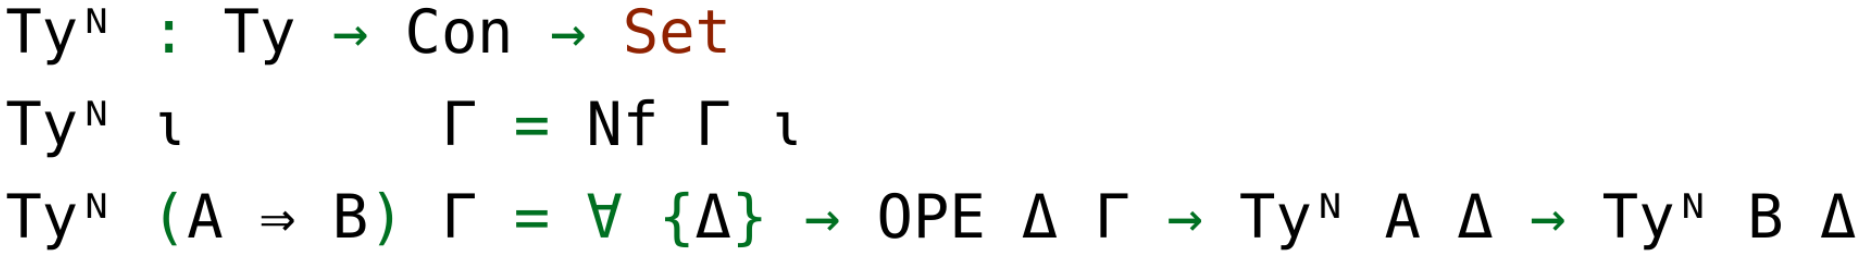
\includegraphics[width=0.7\textwidth]{./images/typed_semantic_set.png}
    \caption{Agda implementation of the typed semantic set from \cite{AgdaNbe}}
    \label{fig:agdaSemanticSet}
\end{figure}

% Differences between Haskell and Agda (presentation)

% The \code{normalise} function should return a \code{NormalForm} with the same type and typing context as the original term, so should have the type signature \code{Expr ctx ty $\rightarrow$ NormalForm ctx ty}. Because \code{reify} is a pure function of the semantic set \code{V}, this set must also be indexed by the typing context and type of the expression to preserve the type information needed to verify a term is well-typed (as seen in the kind signature below). 

In Andras Kovacs' implementation of NbE \cite{AgdaNbe}, the type of the semantic set is determined by the function $\text{Ty}^\text{N}$. This function takes a type and context expression as values, and returns the type of the corresponding semantic set, where \code{Set} can be thought of as kind \code{*}. In Haskell we do not have a way to directly express a function which takes values and returns types. Instead we define the GADT \code{V} which represents the typed semantic set.

\begin{lstlisting}
    data V :: [Ty] -> Ty -> * where 
        Base :: NormalExpr ctx BaseTy -> V ctx BaseTy
        Function :: (forall ctx' .  OPE ctx' ctx -> V ctx' arg -> V ctx' result) 
                 -> V ctx (arg :-> result)
\end{lstlisting}

\code{V} is indexed by a context of kind \code{[Ty]} and a type of kind \code{Ty}, which were value-level function arguments in \ref{fig:agdaSemanticSet}. \code{V} is necessarily indexed by these parameters at the type level since \code{normalise} should return a normal form with the same context and type as the given syntactic expression. \code{reify} is a pure function of the semantic set, so \code{V} must preserve this type-level information. 

$\text{Ty}^\text{N}$ pattern matches on the type argument and is defined in two cases: a base type case and a function case, where the Agda implementation uses $\iota$ for \code{BaseTy}. In our implementation the expression type is not given as a value-level argument that can be pattern matched on, so instead we use constructors to emulate a similar behaviour. From the return type of the constructors we see that values of \code{V} with type \code{BaseTy} can only be created by the \code{Base} constructor. Thus, if we are given a value of type \code{V ctx BaseTy}, GHC can deduce the value takes the form \code{Base n} where \code{n :: NormalExpr ctx Expr}. \code{n} is an inhabitant of the type returned by the Agda implementation in the base type case. 
Similarly, given a value of type \code{V ctx (A :-> B)}, GHC can deduce that the value must have the form \code{Function f}, since only the \code{Function} constructor can produce semantic values with function type. Again, we can extract a semantic value of the correct type since the type of \code{f} is exactly the type specified by the function type case of $\text{Ty}^\text{N}$. Thus, we have successfully mimicked the behaviour of $\text{Ty}^\text{N}$ in Haskell.

% TODO: Limitations of above technique

The argument to the \code{Function} constructor has following the type signature.
\begin{lstlisting}
    forall ctx' . OPE ctx' ctx -> V ctx' arg -> V ctx' result 
\end{lstlisting}

By default, in GHC, there is only have one “level” of polymorphism, where type variables are implicitly universally quantified. However, as seen in \ref{fig:agdaSemanticSet}, we want to treat \code{ctx} as fixed, before quantifying over \code{ctx'}, where we use \code{ctx} instead of $\Gamma$ and \code{ctx'} instead of $\Delta$.
% Those with OPE to original context
To achieve this we use higher-ranked polymorphism with the explicit \code{forall} syntax to delay the quantification of \code{ctx'} until after \code{ctx} has been bound. To enable higher ranked polymorphism, we use the \code{Rank2Types} extension. 

% TODO: Motivation for structure

\section{Evaluation}

In this section we implement the typed \code{eval} function.

\subsection{Environment}

% TODO: Relation to agda

As in the untyped implementation of NbE, during evaluation we need an environment to track bound variables and their associated semantic values. Since our variables have the same structure as de Bruijn indices [CITE IN PAPER] it suffices to use a list as the environment, where the $n$th element of the list corresponds to the variable at de Bruijn index $n$.

% TODO: Motivated by the variable case
% Need extra typing info

\begin{lstlisting}
    data Env :: [Ty] -> [Ty] -> * where
        EmptyEnv :: Env '[] ctxV
        ConsEnv  :: Env ctx ctxV -> V ctxV ty -> Env (ty : ctx) ctxV
\end{lstlisting}

From the constructors, we see that \code{Env} GADT has the same value-level structure as the standard Haskell list. However, we have used GADT syntax to enforce additional restrictions on the types of the elements in the environment. From the kind signature, we see that \code{Env} is indexed by two typing contexts. From the type of \code{ConsEnv}, we see that the first of these tracks the types of the semantic elements stored in the environment. The second typing context is the typing context shared by all semantic values stored in the environment. The motivation for indexing \code{Env} by these typing contexts is due to \code{envLookup} function defined below in \ref{subsect:typedVarCase}.


% Why do ctxs have to match?

\subsection{Variable Case}
\label{subsect:typedVarCase}

Now that we have defined the environment, we are ready to implement the evaluation function \code{eval}.

\begin{lstlisting}
    eval :: Env ctx ctxV -> Expr ctx ty -> V ctxV ty
\end{lstlisting}

As before, we pattern match on each of the three expression constructors. We start with the variable case.

\begin{lstlisting}
    eval env (Var n) = envLookup n env
        where
            envLookup :: Elem ctx ty -> Env ctx ctxV -> V ctxV ty 
            envLookup Head     (ConsEnv _    v) = v
            envLookup (Tail n) (ConsEnv tail _) = envLookup n tail
\end{lstlisting}

As in the untyped case, for variables we simply lookup the semantic value associated with the bound variable from the environment. Since variables are indexed by an \code{Elem} value, \code{envLookup} takes an \code{Elem} value and returns the associated semantic value.

The additional type information allows us to make guarantees about the lookup. Since \code{n} is a value of type \code{Elem ctx ty}, we know that \code{ty} exists somewhere in the list \code{ctx}. Since \code{Env} is also indexed by the same context \code{ctx}, which tracks the types of the semantic values in the environment, it is guaranteed that the semantic value at the corresponding de Bruijn index exists in the environment with type \code{ty}. Thus, \code{envLookup} doesn't have to handle the case where the variable is not in the environment like in the untyped implementation; the types guarantee that all variables possible in the context \code{ctx} are bound in the environment.

Since all semantic values in the environment have the same typing context \code{ctxV}, we can also be sure that the returned semantic value has the context \code{ctxV}.

Note that \code{envLookup} does not pattern matched on the \code{EmptyEnv} case. The types ensure that this case is never required since \code{EmptyEnv} has type \code{Env '[] ctxV}, and there are no inhabitants of the type \code{Elem '[] x} for any \code{x}. Here \code{Elem ctx ty} acts like a pre-condition on \code{envLookup}.

% TODO: Why return into ctxV?

\subsection{Lambda Case}

\begin{lstlisting}
    eval env (Lam body) = Function f 
        where
            f ope v = eval (ConsEnv (strengthenEnv ope env) v) body

    strengthenEnv :: OPE ctxV' ctxV -> Env ctx ctxV -> Env ctx ctxV'
\end{lstlisting}

As in the untyped implementation, in the lambda case \code{eval} returns a semantic function that maps from a semantic argument \code{v} to the body of the lambda. We evaluate the body in an updated environment where we have bound the variable \code{Var Head} to \code{v}. This means the typing context of the returned semantic value will be larger than that of the original expression.

% TODO: Finish above

Since all the semantic values in the environment must have the same typing context, we expand the typing context of each element in the environment to match the typing context \code{ctxV'} of \code{v}. The \code{OPE} argument of \code{f} makes such an expansion possible. By the weakening property of the STLC [CITE], a term will remain well-typed if we expand its typing context with new variable bindings. From a proof perspective, the \code{OPE ctxV' ctxV} argument proves that all the semantic elements of the context  ... 
% Does weakening hold for semantic values?
Note that since all semantic elements of \code{env} have the same context \code{ctxV}, and \code{f} ...

% TODO: Scoped Type variables
% - Show what types are inferred without

% TODO: Remove singletons
\code{strengthenEnv} takes an \code{OPE ctxV' ctxV} and an environment, and returns the same environment where each semantic values has the expanded context \code{ctxV'}

To implement \code{strengthenEnv}, we first build a series of functions for strengthening each constituent part of a semantic value.

\begin{lstlisting}
    strengthenElem :: OPE strong weak -> Elem weak ty -> Elem strong ty
    strengthenElem (Drop ope) v        = Tail (strengthenElem ope v)
    strengthenElem (Keep ope) (Tail v) = Tail (strengthenElem ope v)
    strengthenElem (Keep ope) Head     = Head
\end{lstlisting}

% Q: Can drop Empty case, weak = '[], no elem inhabitiants

First we strengthen \code{Elem} values which represent variables. We use the naming convention \code{OPE strong weak} since \code{strong} could be any context with containing at least the same variable bindings as \code{weak} and more. 
Intuitively the proposition the type of \code{strengthenElem} generates makes sense: if \code{ty} is an element of the context \code{weak}, then it is also an element in any context \code{strong} containing \code{weak}.

% TODO: Explain cases?

\begin{lstlisting} 
    strengthenNormal :: OPE strong weak -> NormalExpr weak ty -> NormalExpr strong ty
    strengthenNormal ope (NormalNeutral n) = NormalNeutral (strengthenNeutral ope n)
    strengthenNormal ope (NormalLam n)     = NormalLam (strengthenNormal (Keep ope) n)

    strengthenNeutral :: OPE strong weak -> NeutralExpr weak ty -> NeutralExpr strong ty
    strengthenNeutral ope (NeutralVar n)   = NeutralVar (strengthenElem ope n)
    strengthenNeutral ope (NeutralApp f a) = NeutralApp (strengthenNeutral ope f) 
                                                        (strengthenNormal ope a) 

\end{lstlisting}

\code{strengthenNeutral} and \code{strengthenNormal} strengthen entire expressions. In the \code{NormalLam} case, type refinement guarentees that the typing context for the body of the lambda binds an variable with type \code{arg}. Hence, we have to expand the given OPE with an additional \code{Keep}. In the \code{strengthenNeutral} case we use \code{strengthenElem} to point variables to their updated indices in the expanded context.

\begin{lstlisting}
    strengthenV :: OPE strong weak -> V weak ty -> V strong ty
    strengthenV ope                      (Base nf) = Base (strengthenNormal ope nf)
    strengthenV (ope :: OPE strong weak) (Function (f :: forall strong . (SingContext strong) => OPE strong weak -> V strong arg -> V strong result)) = Function f' 
        where
            f' :: (SingContext stronger) => OPE stronger strong -> V stronger arg -> V stronger result
            f' ope' = f (composeOPEs ope ope')
\end{lstlisting}

\begin{lstlisting}
    strengthenEnv :: (SingContext c) => OPE c b -> Env a b -> Env a c
    strengthenEnv _   EmptyEnv         = EmptyEnv
    strengthenEnv ope (ConsEnv tail v) = ConsEnv (strengthenEnv ope tail) (strengthenV ope v)
\end{lstlisting}


\begin{lstlisting}
    eval (env :: Env ctx ctxV) (Lam (body :: Expr (arg:ctx) result)) = Function f 
        where
            f :: OPE ctxV' ctxV -> V ctxV' arg -> V ctxV' result
            f ope v = eval (ConsEnv (strengthenEnv ope env) v) body
\end{lstlisting}

\subsection{Application Case}

%TODO: Motivate by pattern matching on type not possible in Haskell

\begin{lstlisting}
    eval env (App f a) = appV (eval env f) (eval env a) 
        where
            appV (Function f') a' = f' (idOPEFromEnv env) a'

            idOPEFromEnv :: (SingContext ctxV) => Env ctx ctxV -> OPE ctxV ctxV
            idOPEFromEnv _ = idOpe 
\end{lstlisting}

\begin{lstlisting}
    class SingContext ctx where
        idOpe :: OPE ctx ctx

    instance SingContext '[] where
        idOpe = Empty

    instance (SingContext xs, SingTy x) => SingContext (x:xs) where
        idOpe = Keep idOpe
\end{lstlisting}

%TODO Include code link

\section{Reification}

\begin{lstlisting}
    reify :: V ctx ty -> NormalExpr ctx ty
    reify (Base nf)    = nf
    reify (Function f) = NormalLam (reify (f ope (evalNeutral (NeutralVar Head)))) 
        where
            ope = weakenContext (Function f)

            weakenContext :: (SingContext ctx) => V ctx ty -> OPE (x:ctx) ctx
            weakenContext _ = wk 

    evalNeutral :: (SingTy ty, SingContext ctx) => NeutralExpr ctx ty -> V ctx ty
    evalNeutral = evalNeutral' singTy

    evalNeutral' :: (SingContext ctx) => STy ty -> NeutralExpr ctx ty -> V ctx ty
    evalNeutral' SBaseTy       n                                       = Base (NormalNeutral n)  
    evalNeutral' (SArrow _ _)  (n :: NeutralExpr ctx (arg :-> result)) = Function f 
        where
            f :: (SingContext strongerCtx) => OPE strongerCtx ctx -> V strongerCtx arg -> V strongerCtx result
            f ope v = evalNeutral (NeutralApp (strengthenNeutral ope n) (reify v))
\end{lstlisting}

% TODO: Motivate evalNeutral and rename, contrast with standard eval

\begin{lstlisting}
    data STy :: Ty -> * where
        SBaseTy :: STy BaseTy
        SArrow  :: (SingTy a, SingTy b) => STy a -> STy b -> STy (a :-> b)

    class SingTy a where
        singTy :: STy a 

    instance SingTy 'BaseTy where
        singTy = SBaseTy

    instance (SingTy a, SingTy b) => SingTy (a :-> b) where
        singTy = SArrow singTy singTy
\end{lstlisting}

\begin{lstlisting}
    class SingContext ctx where
        idOpe :: OPE ctx ctx
        wk :: OPE (x:ctx) ctx
        wk = Drop idOpe
\end{lstlisting}

\section{Normalisation}

\begin{lstlisting}
    normalise :: (SingContext ctx) => Expr ctx ty -> NormalExpr ctx ty
    normalise = reify . eval initialEnv
\end{lstlisting}

\begin{lstlisting}
    class SingContext ctx where
        idOpe :: OPE ctx ctx
        wk :: OPE (x:ctx) ctx
        wk = Drop idOpe
        initialEnv :: Env ctx ctx

    instance SingContext '[] where
        idOpe = Empty
        initialEnv = EmptyEnv

    instance (SingContext xs, SingTy x) => SingContext (x:xs) where
        idOpe = Keep idOpe
        initialEnv = ConsEnv (strengthenEnv wk initialEnv) (evalNeutral (NeutralVar Head))
\end{lstlisting}

\section{For presentation}

\begin{lstlisting}
    evalNeutral :: (SingTy ty) => NeutralExpr ctx ty -> V ctx ty
    evalNeutral = evalNeutral' singTy

    evalNeutral' :: STy ty -> NeutralExpr ctx ty -> V ctx ty
    evalNeutral' SBaseTy      n = ...
    evalNeutral' (SArrow _ _) n = ...

    evalNeutral :: STy ty -> NeutralExpr ctx ty -> V ctx ty
    evalNeutral SBaseTy      n = ...
    evalNeutral (SArrow _ _) n = ...

    eval (env :: Env ctx ctxV) (Lam (body :: Expr (arg:ctx) result)) = Function f 
        where
            f :: OPE ctxV' ctxV -> V ctxV' arg -> V ctxV' result
            f ope v = ...

    eval env (Lam body) = Function f 
        where
            f ope v = ...
\end{lstlisting}

\section{Notes}

Investigation: Are GADTs in Haskell powerful enough? Types are erased at runtime so true dependent typing not part of Haskell (programs at type level)

Advantage over ADTs: type refinement by constructor

Poissible to erase all type information, NbE on Untyped
Issue: No proof that type preserved 
Solution: Track types as do evaluation - nbe program itself proof that types preserved (subject reduction parallel?)

Started by implementing same as untyped

Main difference in semantics (V := a -> b | Neutral) 
\cite{slides}

problem: Need to strengthen context evaluating body (eval Lam case)
\subsection{Solution: Order Preserving Embeddings (OPEs)}

Following implementation in Agda \cite{AgdaNbe}, agda has full dependent types (type system more powerful) - adapt for haskell, how nicely? 

if a term well typed for one context, also well typed for any longer one

A value of type 'OPE strong weak' can derive weak from strong by dropping elements from context

OPE is a relation on typing contexts

\subsection{Semantic set}

Defintion of V using OPEs - Haskell vs agda

Need to quantify over 'strong' in function - OPE strong weak is guarentee that strong is a stronger context than weak (if quantified at start end up with values where weak stronger than strong) - need rank2 types extension for nested quantification

Helper functions (composition, strengthing relative to OPE) - explain derivations

\subsection{implementing Eval}

Defintion of environment (maps expressions in syntax context ctx to values in semantics with context ctxV)

problem: in app case how to we get identity OPE for semantic context?

But types erased at compile time to make Haskell efficient

How to generate a value at runtime dependent on type erased at compile time

dependent pattern match \cite{SingletonsGuide}

\subsection{Solution: Singleton pattern}

Method of Type to value known as reflection \cite{SingletonsGuide}

Idea: Create value-level tags for types - singleton types correspond type we're interested in, inhabited by only one value for each case

Examples: Reify case analysis, Ty reflection, Context reflection

Explicitly passing as value to pattern match on

Generate implictly using typeclass, use class constraint to imiplictly pass down ability to use contex methods through function calls.
Is it a good idea to have class constraints in the GADTs/Syntax definitions?

Implementation in class vs full reflection - test this for speed?

problem : Inferring Any for ctxV (why?)

solution: scoped type variables - universally quantified variables used in type expressions bind over 'where' clause

(More usefully) can 'unpack' refined GADT types so that can create type definitions using refined types.

Analysis:

Have to specify type when normaling for correct eta-expansion (eta-long form)

Qs:
How does locally nameless work in sematics?
How does ctxV work in Env?
